\documentclass[../main.tex]{subfiles}

\begin{document}
\قسمت{آقای یا خانم؟}

\زیرقسمت{مقدمه}
\پاراگراف{}
یکی از سخترین کارها در کلاس و مخصوصا کلاس‌های آنلاین استفاده صحیح از پیشوندهای آقای و خانم می‌باشد.
مثلا شما در لیست اسم پرهام الوانی را می‌بینید و نمی‌دانید باید بگویید آقای الوانی یا خانم الوانی.
در این تمرین قصد داریم وب‌سایتی طراحی کنیم که در این امر مهم اساتید را یاری دهد.

\زیرقسمت{وبگاه}
\پاراگراف{}
این وبگاه از شِمای زیر پیروی می‌کند. یک پس زمینه تمام صفحه را در بر گرفته است و در میان آن یک مستطیل شفاف قرار گرفته است.
دقت داشته باشید شفافیت نباید به قدری باشد که متن‌های درون مستطیل خوانایی نداشته باشند.

\begin{figure}[h]
  \centering
  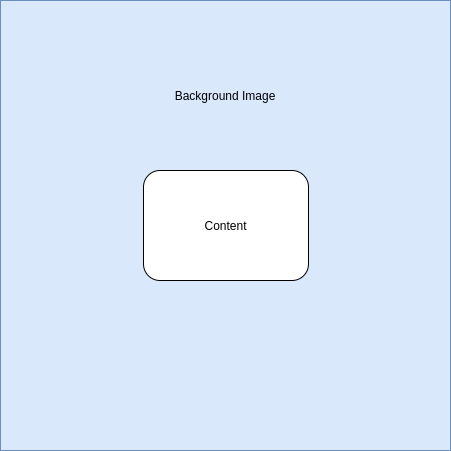
\includegraphics[scale=0.25]{./genderize-top-level}
  \caption{طراحی سطح بالا}
\end{figure}

\پاراگراف{}
مستطیل میانی تمامی محتویات قابل نمایش شما را می‌بایست شامل شود. این مستطیل می‌بایست تنها به اندازه محتویات باشد اما برای نمایش زیباتر آن از لایه‌گذاری\پانویس{padding} استفاده کنید.
محتوای شما از دو قسمت تشکیل شده است که به صورت افقی کنار یکدیگر قرار گرفته‌اند. قسمت اول یک فرم است که خود از دو ورودی تشکیل شده است. وروردی اول به شکل متنی بوده و کاربر اسم مورد نظر را وارد می‌کند.
ورودی دوم به شکل دو دکمه رادیویی است که به کاربر می‌کند اگر از پیش جواب را می‌داند آن را وارد کرده و این جواب برای آینده ذخیره می‌شود. در مورد جواب‌های ذخیره شده در ادامه بیشتر صحبت خواهد شد.

\begin{figure}[h]
  \centering
  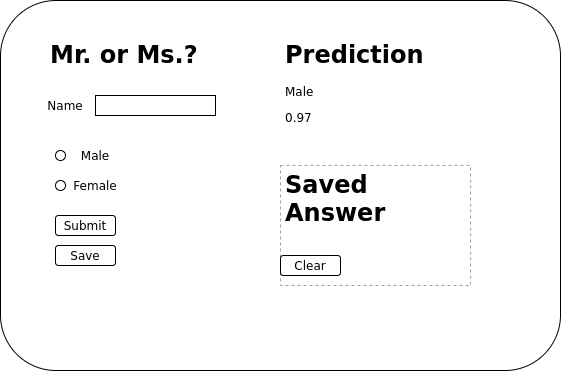
\includegraphics[scale=0.25]{./genderize-content}
  \caption{طراحی مستطیل محتوا}
\end{figure}

\پاراگراف{}
پس از پر کردن فرم کاربر گزینه درخواست\پانویس{submit} را زده و به این درخواست ایشان ارسال می‌شود. برای پیش‌بینی جنسیت اسم داده شده از وبگاه زیر استفاده می‌کنیم:

\begin{latin}\begin{center}
https://api.genderize.io/?name=hassan
\end{center}\end{latin}

شما نام را در قالب یک رشته تقاضا\پانویس{query string} برای این وبگاه ارسال می‌کنید و در نهایت حاصل پیش‌بینی را به کاربر نمایش می‌دهید. خروجی این درخواست به شکل زیر می‌باشد:

\begin{latin}
\begin{minted}[bgcolor=LightGray]{http}
{
  "name":"hassan",
  "gender":"male",
  "probability":0.97,
  "count":49197
}
\end{minted}
\end{latin}

\شروع{امتیازی}
ممکن است به دلیل شبکه ارسال درخواست به خطا بخورد یا اینکه این وبگاه نتواند برای یک نام پیش‌بینی داشته باشد (برای نمونه این وبگاه برای نام ``محمد حسین'' پیش‌بینی ندارد). شما می‌بایست این خطاها را با نمایش پیام خطا به کاربر رسیدگی کنید. دقت داشته باشید که نمایش می‌بایست در وبگاه شما صورت بگیرد و نمایش در کنسول مرورگر مجاز نمی‌باشد.
\پایان{امتیازی}

\زیرقسمت{جواب‌های ذخیره شده}
زمان‌هایی وجود دارد که وبگاه پیش‌بینی اشتباه انجام می‌دهد، در این صورت می‌توان با پرس از دانشجو به پاسخ صحیح رسید. در این صورت این سامانه می‌بایست توانایی ذخیره کردن پاسخ صحیح را داشته باشد. برای ذخیره کردن پاسخ صحیح یک راه استفاده از کوکی‌ها می‌باشد. در نهایت اگر اسم وارد شده در قالب کوکی موجود باشد شما می‌بایست پاسخ ذخیره شده را نیز به کاربر نمایش دهید.

\شروع{امتیازی}
می‌توانید به جای استفاده از کوکی‌ها از \متن‌لاتین{local storage} استفاده کنید. برای آشنایی بیشتر می‌توانید از وبگاه زیر کمک بگیرید.


\begin{latin}\begin{center}
https://developer.mozilla.org/en-US/docs/Web/API/Window/localStorage
\end{center}\end{latin}

\پایان{امتیازی}

\زیرقسمت{نکات پیاده‌سازی}

\شروع{فقرات}
    \فقره برای کدهایتان از کامنت استفاده کنید. توضیح کارکرد بلاک‌های \متن‌لاتین{CSS} اجباری می‌باشد. توابعی و قطعات کد جاوا اسکریپت نیز می‌بایست حداقل یک خط کامنت داشته باشند.
    \فقره کامنت فارسی یا انگلیسی موردی ندارد اما از فینگلیش (!) نوشتن پرهیز کنید.
    \فقره استفاده از کتابخانه‌ها در پروژه مجاز \متن‌سیاه{نمی‌باشد}.
    \فقره استفاده یکی از چهارچوب‌های \متن‌لاتین{react}، \متن‌لاتین{vue} و \متن‌لاتین{angular} نمره امتیازی دارد.
    \فقره از آنجایی که این پروژه در قالب \متن‌سیاه{امتحان میانترم} می‌باشد از تغییر دادن صورت مساله یا انجام موارد خارج از موارد مطرح شده خودداری کنید.
\پایان{فقرات}

\زیرقسمت{پرسش‌های متداول}

هنوز سوالی پرسیده نشده است، صورت پروژه در مهلت انجام پروژه بر پایه سوالات شما به روزرسانی خواهد شد.
%\شروع{شمارش}
%\پایان{شمارش}

\end{document}
